\subsection{Evaluaci\'on de desempe\~no del software en pruebas iniciales 2}
    En las pruebas iniciales ya en entornos controlados y de un
        tama\~no bastante reducido, se hizo del conocimiento de
        algunos detalles que surgen de la implementaci\'on de algunas
        funcionalidades, las cuales fueron revisadas a detalle.
    \vskip 0.5cm
    Como se mencion\'o anteriormente, como medida de
        desempe\~no se utilizar\'a el tiempo que tarda el software entre
        el cambio de generaci\'on entre una evaluaci\'on de las reglas y
        otra. A diferencia de las anteriores evaluaciones, en este caso
        al ya implementar un mapa que est\'a basado ya en una
        locaci\'on en espec\'ifico, se tiene que realizar una
        configuraci\'on la cual sea lo m\'as aproximado a su locaci\'on
        en el mundo real.
    \vskip 0.5cm
    Las siguientes pruebas corresponden a un mapa el cual se
        tiene por defecto y representa en el \'area en la cual el robot
        fue colocado en la vida real para poder comprobar el
        funcionamiento del seguimiento de la ruta. Es importante
        recalcar que las pruebas se realizan en ambos sistemas
        operativos, los cuales son, como es asumido desde el inicio, 
        el sistema operativo de Windows y Linux, usando como
        principal distribuci\'on la de Ubuntu en el caso de Linux. Esto se
        se puede ver en las Figuras \ref{fig:Ruta 47} - \ref{fig:Ruta 57}.
    \vskip 0.5cm
    %figura
    \begin{figure}[htbp]
        \centering
        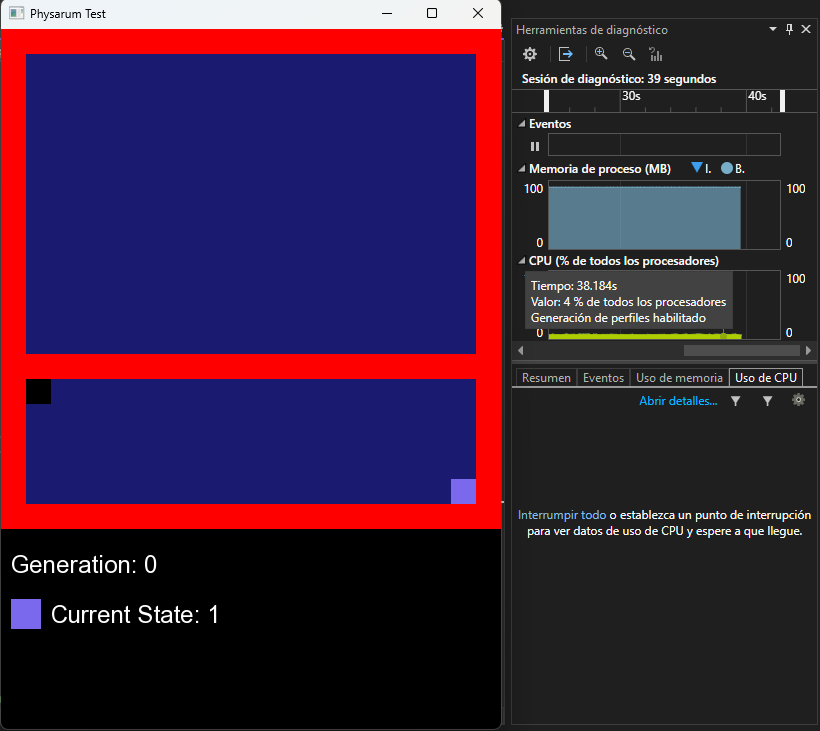
\includegraphics[width=0.5\textwidth]{./images/Pruebas/simulador/image047.png}
        \caption{Estado inicial con una barrera simulando un cuadro cerrado en Windows}
        \label{fig:Ruta 47}
    \end{figure}
    \vskip 0.5cm
    %figura
    \begin{figure}[htbp]
        \centering
        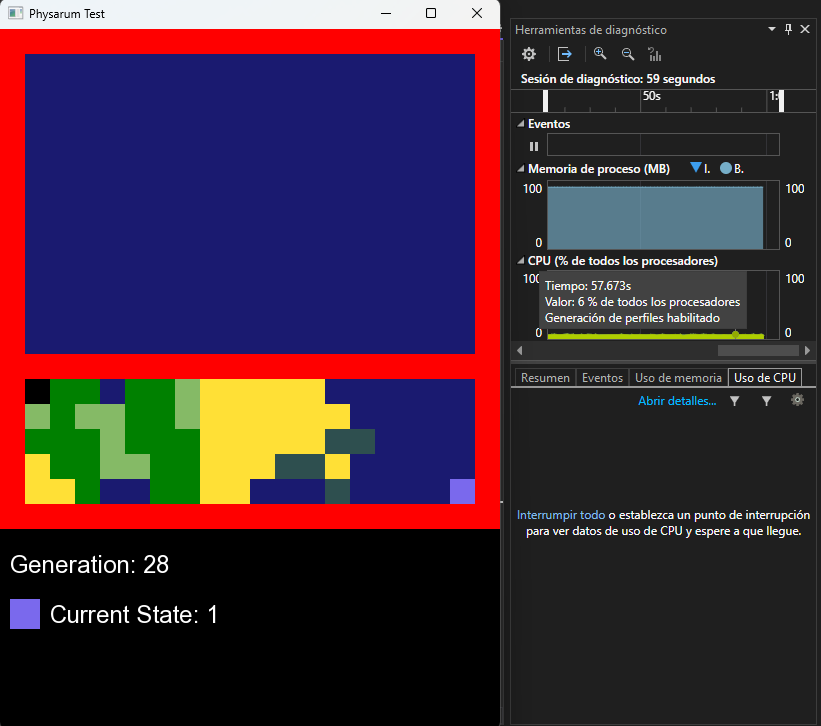
\includegraphics[width=0.5\textwidth]{./images/Pruebas/simulador/image049.png}
        \caption{Rendimiento de la aplicaci\'on en un entorno cerrado y durante la expansi\'on del Physarum en Windows}
        \label{fig:Ruta 49}
    \end{figure}
    \vskip 0.5cm
    %figura
    \begin{figure}[htbp]
        \centering
        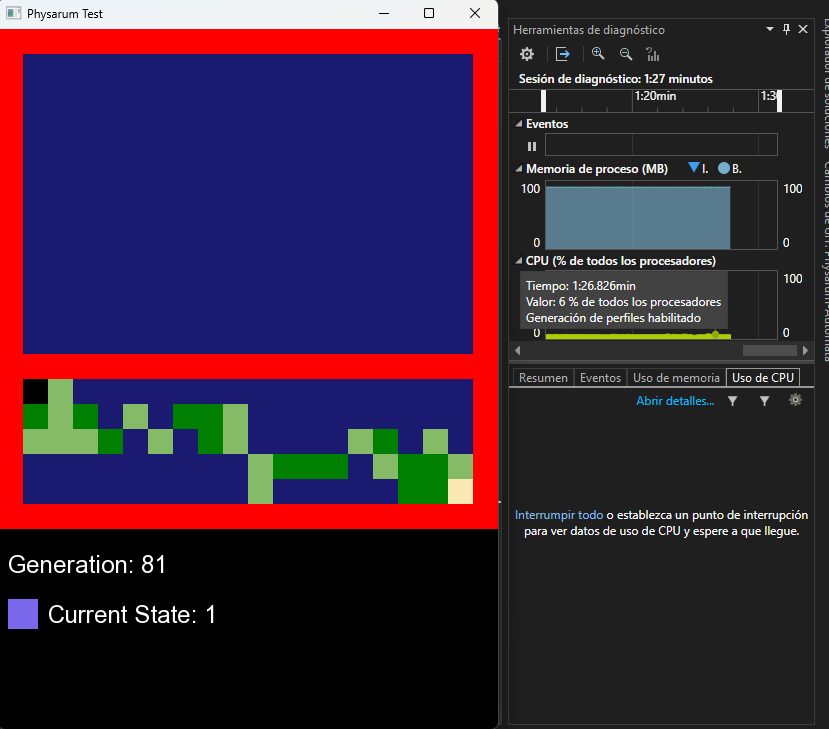
\includegraphics[width=0.5\textwidth]{./images/Pruebas/simulador/image051.png}
        \caption{Rendimiento al generar la ruta con el Physarum Windows}
        \label{fig:Ruta 51}
    \end{figure}
    \vskip 0.5cm
    %figura
    \begin{figure}[htbp]
        \centering
        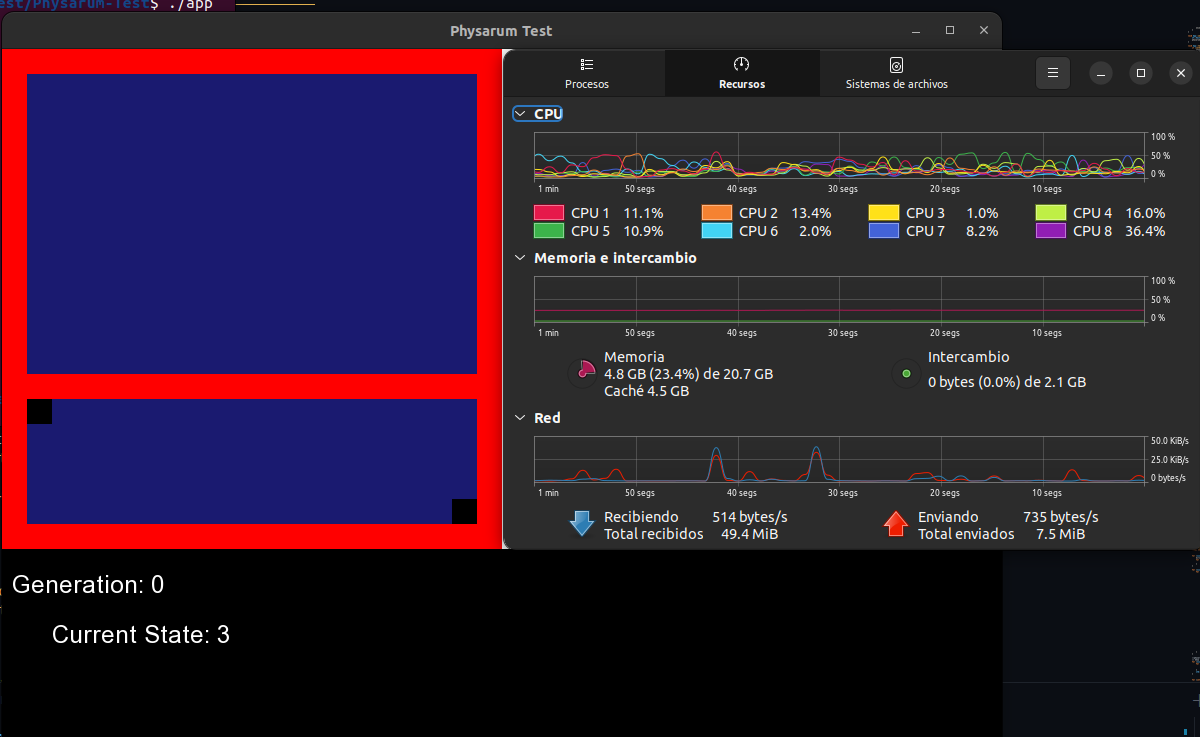
\includegraphics[width=0.5\textwidth]{./images/Pruebas/simulador/image053.png}
        \caption{Rendimiento de la aplicaci\'on durante el establecimiento del estado inicial en Linux}
        \label{fig:Ruta 53}
    \end{figure}
    \vskip 0.5cm
    %figura
    \begin{figure}[htbp]
        \centering
        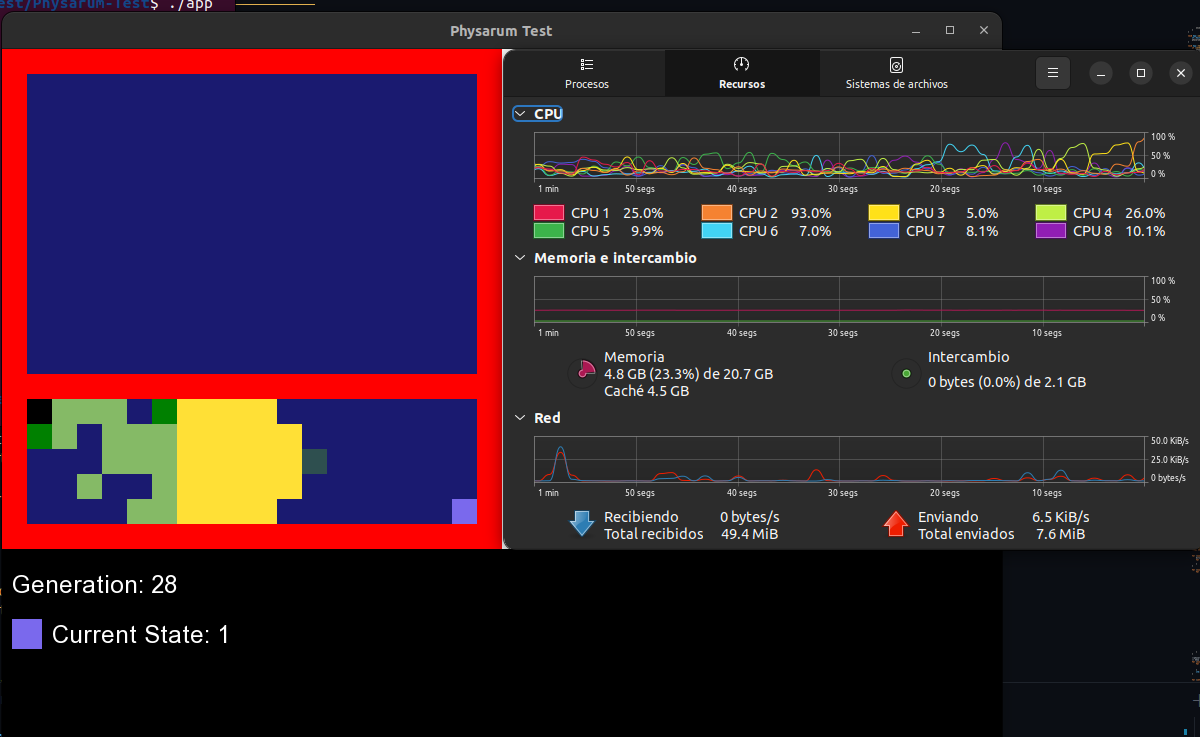
\includegraphics[width=0.5\textwidth]{./images/Pruebas/simulador/image055.png}
        \caption{Rendimiento de la aplicaci\'on durante la expansi\'on del Physarum en Linux}
        \label{fig:Ruta 55}
    \end{figure}
    \vskip 0.5cm
    %figura
    \begin{figure}[htbp]
        \centering
        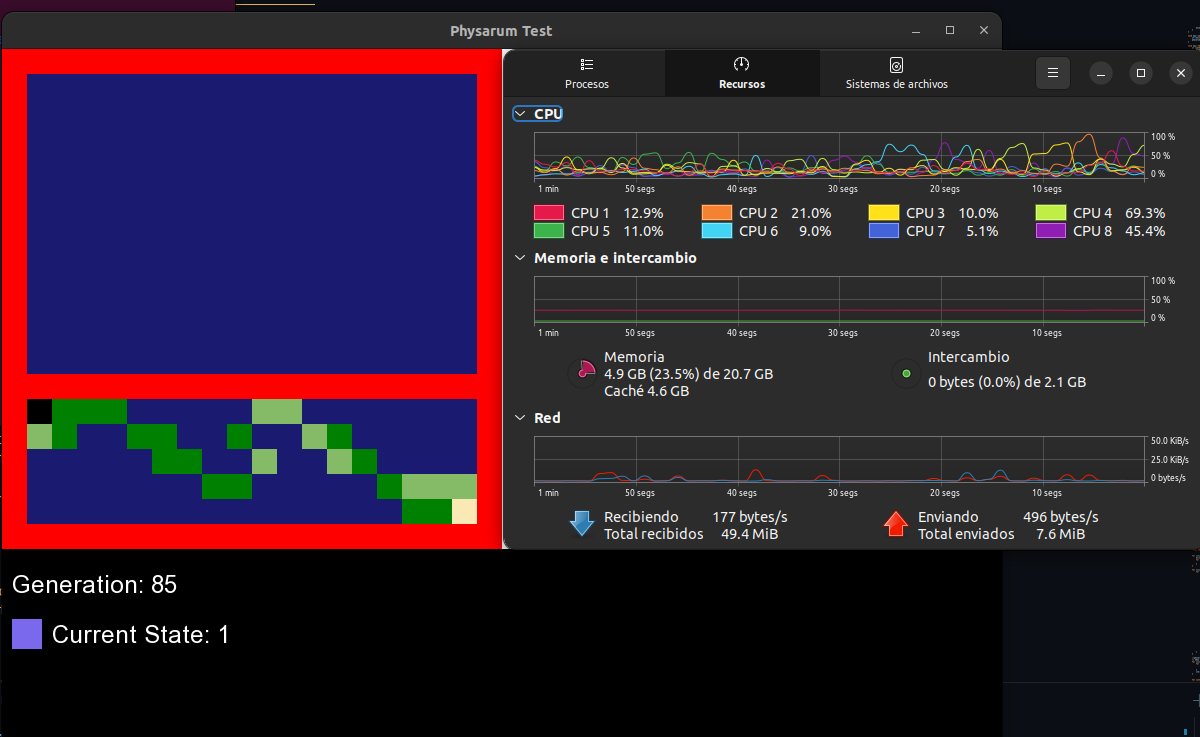
\includegraphics[width=0.5\textwidth]{./images/Pruebas/simulador/image057.png}
        \caption{Rendimiento al generar la ruta con el Physarum en Linux}
        \label{fig:Ruta 57}
    \end{figure}